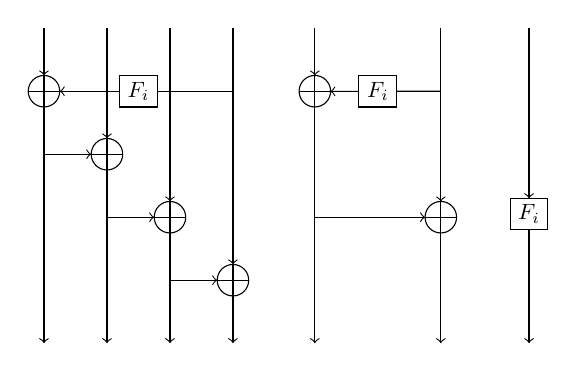
\begin{tikzpicture}[scale=0.8]

\tikzstyle{every node}=[transform shape];

\begin{scope}[xshift=-4cm, shift={(-0.5,-1)}]
\draw[->] (0.5,0) -- ++(0,-1+0.25);
\draw[] (0.5,-1) circle (0.25);
\draw[] (0.25,-1) -- ++(0.5,0);  
\draw[->] (3.5,-1) -- ++(-3+0.25,0);
\draw[fill=white] (1.5+0.2,-1-0.25) rectangle node {\textsf{$F_{i}$}} ++(1-0.4,0.5);
\draw[->] (0.5,-1+0.25) --  ++(0,-4.5+0.25);

\draw[->] (1.5,0) -- ++(0,-2+0.25);
\draw[->] (1.5,-2+0.25) -- ++(0,-3.25);
\draw[->] (0.5,-2) -- ++(1-0.25,0);
\draw[]   (1.5,-2) circle (0.25);
\draw[]   (1.25,-2) -- ++(0.5,0);  

\draw[->] (2.5,0) -- ++(0,-3+0.25);
\draw[->] (2.5,-3+0.25) -- ++(0,-2.25);
\draw[->] (1.5,-3) -- ++(1-0.25,0);
\draw[]   (2.5,-3) circle (0.25);
\draw[]   (2.25,-3) -- ++(0.5,0);  

\draw[->] (3.5,0) -- ++(0,-4+0.25);
\draw[->] (3.5,-4+0.25) -- ++(0,-1.25);
\draw[->] (2.5,-4) -- ++(1-0.25,0);
\draw[]   (3.5,-4) circle (0.25);
\draw[]   (3.25,-4) -- ++(0.5,0);  
\end{scope}

\begin{scope}[xshift=1cm, shift={(-1.2,-1)}]
\draw[->] (0.5,0) -- ++(0,-1+0.25);
\draw[] (0.5,-1) circle (0.25);
\draw[] (0.25,-1) -- ++(0.5,0);  
\draw[->] (2.5,-1) --++(-1.7544,-0.0019);
\draw[fill=white] (1.2,-1-0.25) rectangle node {\textsf{$F_{i}$}} ++(1-0.4,0.5);
\draw[->] (0.5,-1+0.25) --  ++(0,-4.5+0.25);

\draw[->] (0.5,-3)--(2.25,-3);
\draw[->] (2.5,0) -- ++(0,-3+0.25);
\draw[->] (2.5,-3+0.25) -- ++(0,-2.25);
\draw[]   (2.5,-3) circle (0.25);
\draw[]   (2.25,-3) -- ++(0.5,0);  
\end{scope}

\draw [->](3.7,-1) -- (3.7,-3.7);
\draw[fill=white] (3.4,-4.2) rectangle node {\textsf{$F_{i}$}} (4,-3.7);
\draw [->](3.7,-4.2) -- (3.7,-6);
\end{tikzpicture}        